\documentclass[pdftex,12pt,a4paper]{article}
\usepackage[pdftex]{graphicx}
\usepackage{xcolor}
\usepackage{marginnote}
\usepackage{enumitem}
\usepackage[bottom=1.5cm, outer=5cm, inner=2cm, heightrounded,
marginparwidth=4cm, marginparsep=0.5cm]{geometry}

\begin{document}
    % Custom title page
    \begin{titlepage}
        \begin{center}
            
\includegraphics[width=5cm]{figures/kulogo}\\[1cm]
            {\Large \bfseries
                Spring 2014\\
                Computer Networks\\
                CMPE323\\[1cm]
            }
            {\large \bfseries
                \noindent Laboratory Experiment No. 5: Introduction to User
                Datagram Protocol (UDP)\\[1cm]
            }
        \end{center}

        \noindent \textbf{Aims and Objectives:}
            \begin{itemize}[leftmargin=4cm]
                \item Introduce students to UDP, a common layer 4 protocol.
                \item Allow students to manually craft UDP datagrams (including
                    lower layer protocols that they have learned in past labs).
                \item Practically verify the correct behavior according to the
                    UDP standard (IETF 768).
            \end{itemize}
            \vspace{0.5cm}

        \noindent \textbf{Materials Required:}
            \begin{itemize}[leftmargin=4cm]
                \item IP routers,
                \item Ethernet switches,
                \item PCs with Ethernet adapters,
                \item and straight-through/crossover/rollover cables.
            \end{itemize}
            \vspace{0.5cm}

        \noindent \textbf{Change Log:}
            \begin{itemize}[leftmargin=4cm]
                \item 25-3-2014: original document -- mkhonji.
                \item 26-3-2014: fixing language typos -- mkhonji.
            \end{itemize}
    \end{titlepage}
    \newpage

    % Lab script content
    \section{Introduction}
        \begin{figure}[tbh]
                    \begin{center}
                    \begin{verbatim}
               0      7 8     15 16    23 24    31
               +--------+--------+--------+--------+
               | Source Port     | Destination Port|
               +--------+--------+--------+--------+
               |     Length      |    Checksum     |
               +--------+--------+--------+--------+
               |          data octets ...
               +---------------- ...\end{verbatim}
            \end{center}
            \vspace{-15pt}
            \caption{UDP Header Format --- Source: RFC768.}
            \label{fig:udp}
            \vspace{10pt}
        \end{figure}

        \begin{figure}[tbh]
                    \begin{center}
                    \begin{verbatim}
               0      7 8     15 16    23 24    31
               +--------+--------+--------+--------+
               |          source address           |
               +--------+--------+--------+--------+
               |       destination address         |
               +--------+--------+--------+--------+
               |  zero  |protocol|   UDP length    |
               +-----------------------------------+\end{verbatim}
            \end{center}
            \vspace{-15pt}
            \caption{Pseudo IP header used in UDP checksum calculation ---
            Source: RFC768.}
            \label{fig:udpsip}
        \end{figure}

        In the previous lab, we discussed how the Internet Protocol (IP) and
        Classless Inter-Domain Routing (CIDR) allow end-to-end reachability
        across multiple layer 2 networks. 

        However, what we did not discuss so far is: how can applications know
        which messages are for them? 
        
        For example, a node in a network (e.g. a computer running Linux or
        Windows) can have multiple applications running on it (e.g. Firefox,
        IE, IRC clients, \ldots). When such node receives network datagrams,
        how can the node know which datagram is for which application? E.g.
        should the datagram go to (say) Firefox (a HTTP client), irssi (an IRC client), Thunderbird
        (a mail client), \ldots?

        In this lab, we discuss a simple protocol that does exactly that:
        allowing sender and receiver nodes determine which application is for
        which datagram.

        The mechanism that is used is quite simple: for every datagram that you
        send, you add a new header (called the UDP header) which primarily
        includes to fields:
        \begin{itemize}
            \item Destination port number: a number that destination
                application is expected to be listening on. 
            \item Source port number: a number that source 
                application is listening on. This is used by the source
                application to tell the remove application which source the
                source application is listening on. However, in scenarios were a
                source application does not expect a reply, this field is set
                to 0.
        \end{itemize}

        Figure \ref{fig:udp} presents the structure of the UDP header, which
        has 16 bit source port number, 16 bit destination port number, 16 bit
        length (UDP header + UDP payload), and 16 bit checksum (one's
        complement of one's complement sum of 16 bit words of the pseudo IP
        header + UDP header + UDP payload + 0 pads if needed). Figure
        \ref{fig:udpsip} shows the structure of the pseudo IP header. Note:
        when the checksum in the UDP header is set to 0, it is considered as
        disabled (RFC768).

        For example, consider the two network nodes (PCs) $A$ and $B$ as
        follows:
        \begin{itemize}
            \item $A$ has the IP address $IP_A$ and runs the
                applications $a_{1}, a_{2}$ and $a_{3}$ which listen
                on UDP ports $p_1, p_2$ and $p_3$ respectively.
            \item $B$ has the IP address $IP_B$ and runs the
                applications $a_{1}, a_{2}$ and $a_{3}$ which listen
                on UDP ports $p_1, p_2$ and $p_3$ respectively.
        \end{itemize}

        If the application $a_1$ on node $A$ wishes to send a message to
        application $a_1$ on node $B$, then $A$ has to send an IP packet with
        the destination IP address $IP_B$ and the destination UDP port $p_1$


    \section{Lab Preparation}
        \begin{enumerate}
            \item Connect a PC to the routers console port using a rollover
                cable\footnote{If using Linux: \texttt{screen /dev/ttySx} were
                \texttt{x} is the
                serial interfaces ID that is connected to the console
                cable. If using Windows: Use Hyperterminal or Putty to
                connect to \texttt{COMx} ports.}.
            \item Erase the configuration of the
                routers\footnote{\texttt{enable}, \texttt{erase
                startup-config}, \texttt{reload}, and make sure to answer
                \texttt{no} to all yes/no questions while hitting
                \emph{enter} for all \texttt{confirm} prompts.}.
            \item Connect a PC to the switches console ports using rollover
                cables.
            \item Erase the configuration of the
                switch\footnote{\texttt{enable}, \texttt{erase startup-config},
                \texttt{delete vlan.dat}, \texttt{reload}, and answer
                \texttt{no} to all yes/no questions while hitting
                \emph{enter} for all \texttt{confirm} prompts.}.
            \item Run Wireshark on all involved lab PCs as depicted in Figure
                \ref{fig:labtop}.
            \item Physically connect the lab as depicted in Figure \ref{fig:labtop}.
            \item Configure the interfaces:
                \begin{itemize}
                    \item Configure\footnote{\texttt{enable}, \texttt{configure
                        terminal}, \texttt{interface Gi0/0}, \texttt{ip address
                        10.0.0.1 255.255.255.0}.} \texttt{R1}'s interfaces as follows:
                        \begin{itemize}
                            \item GigabitEthernet 0/0: IPv4 address 10.0.12.1,
                                subnet mask 255.255.255.0.
                            \item GigabitEthernet 0/1: IPv4 address 10.0.1.1,
                                subnet mask 255.255.255.0.
                        \end{itemize}
                    \item Configure \texttt{R2}'s interfaces as follows:
                        \begin{itemize}
                            \item GigabitEthernet 0/0: IPv4 address 10.0.12.2,
                                subnet mask 255.255.255.0.
                            \item GigabitEthernet 0/1: IPv4 address 10.0.2.1,
                                subnet mask 255.255.255.0.
                        \end{itemize}
                    \item Configure\footnote{\texttt{ifconfig eth0 10.0.1.2/24}}
                        \texttt{\texttt{PC1}}'s interfaces as follows:
                        \begin{itemize}
                            \item eth0: IPv4 address 10.0.1.2,
                                subnet mask 255.255.255.0.
                        \end{itemize}
                    \item Configure \texttt{\texttt{PC2}}'s interfaces as follows:
                        \begin{itemize}
                            \item eth0: IPv4 address 10.0.2.2,
                                subnet mask 255.255.255.0.
                        \end{itemize}
                \end{itemize}
                
            \item Then add the IP routing tables as follows:
                \begin{itemize}
                    \item For R1: \texttt{ip route 10.0.2.0 255.255.255.0
                        10.0.12.2}
                    \item For R2: \texttt{ip route 10.0.1.0 255.255.255.0
                        10.0.12.1}
                    \item For PC1: \texttt{route add -net 0.0.0.0/0 gw
                        10.0.1.1}
                    \item For PC2: \texttt{route add -net 0.0.0.0/0 gw
                                10.0.2.1}
                \end{itemize}
            \item Test connectivity using the \texttt{ping} command to send
                ICMP Echo messages to PCs in other networks and receive the
                respective ICMP Echo-Reply messages back.
        \end{enumerate}

        \begin{figure}[tbh]
            \centering
            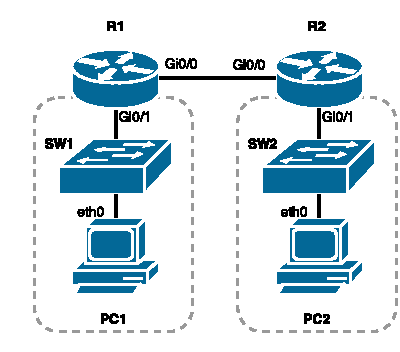
\includegraphics[width=0.6\textwidth]{figures/labtop}
            \caption{Physical lab topology.}
            \label{fig:labtop}
        \end{figure}

    \section{Lab experiments}
        \begin{flushright}
            \textbf{[100 points]}\marginnote{\small \textbf{Note:} When done, show your
            work to the lab engineer for grading purposes.}
        \end{flushright}

        Using the \texttt{nc}\footnote{\texttt{nc -l -p 100 -s 10.0.1.2}}
        command run three applications on PC1 that listen on UDP ports as
        follows:
        \begin{itemize}
            \item Application 1: listen on IP 10.0.1.2 and UDP port 100.
            \item Application 2: listen on IP 10.0.1.2 and UDP port 200.
            \item Application 3: listen on IP 10.0.1.2 and UDP port 300
        \end{itemize}

        Then, using the provided tools (macframesender.c, or scapy) send the
        following UDP messages:
        \begin{itemize}
            \item Message 1: "Hello" from PC2 to PC1's \texttt{nc} that is
                listening on port 100.
            \item Message 2: "Hello" from PC2 to PC1's \texttt{nc} that is
                listening on port 200.
            \item Message 3: "Hello" from PC2 to PC1's \texttt{nc} that is
                listening on port 300.
        \end{itemize}

        \textbf{NOTE:} the tool \texttt{nc} will not accept subsequent
        connections from \emph{other} source IP addresses and source port
        numbers after it is used by some source IP and source port. Note that
        this is only a limitation in \texttt{nc} and it is easy to code UDP
        servers that accept connections from multiple clients.

\end{document}
